\section{Zielsetzung}
\label{sec:Zielsetzung}
Die effektive Masse beschreibt in der Festkörperphysik die scheinbare Masse von Teilchen in einem Kristall. In diesem Versuch wird die effektive Masse der Leitungselektronen von
n-dotiertem Galliumarsenid (n-GaAs) mithife des Effekts der Faradayrotation bestimmt. Der Faraday-Effekt bezeichnet die Drehung der Polarisationsebene von linear polarisiertem Licht
beim Durchgang durch ein Medium in einem Magnetfeld.

\section{Theorie}
\label{sec:Theorie}
\subsection{Bandstruktur}
\label{subsec:Bandstruktur}
Das Konzept der Bandstruktur ist elementarer Bestandteil der Festkörperphysik und beschreibt die Überlagerung diskreter Energieniveaus von Teilchen in einem Kristall. Das Valenzband
entspricht den bei $T=\qty{0}{\kelvin}$ höchstem besetzten Energieband. Befinden sich freie Elektronen im darüber liegenden Leitungsband wird das Material leitend.
Es ergibt sich für verschiedene Materialien eine Struktur, die bestimmte Eigenschaften definiert. So ergibt es sich, dass Materialien mit einer großen Bandlücke zwischen 
Valenz- und Leitungsband einem Isolator entsprechen. Umgekehrt sind Materialien mit keiner Bandlücke Leiter.

Materialien mit einer relativ kleinen Bandlücke von etwa $\symup{\Delta}E_{\text{gap}}=\qtyrange{0}{6}{\electronvolt}$ weisen nochmal andere Eigenschaften auf und werden als Halbleiter
bezeichnet. Am absoluten Temperaturnullpunkt von $T=\qty{0}{\kelvin}$ ist ein Halbleiter nichtleitend, die Fermienergie liegt demnach in der Bandlücke. Für Raumtemperaturen liegt die
thermische Energie der Elektronen bei rund $E_{\text{therm.}}=\qty{26}{\milli\electronvolt}$. Hat ein Halbleiter eine Bandlücke in etwa diesem Energiebereich, treten Elektronen in das 
Leitungsband über und das Material wird leitend.

Die Bandlücke von dem in diesem Versuch verwendetem Galliumarsenid beträgt $E_{\text{gap, GaAs}} = \qty{1,42}{\electronvolt}$, somit befinden sich bei Raumtemperatur sehr wenig 
Elektronen im Leitungsband und die Leitfähigkeit ist entsprechend gering. Durch das Einbringen von Fremdatomen kann ein DOTIERBAND 

\begin{figure}
    \centering
    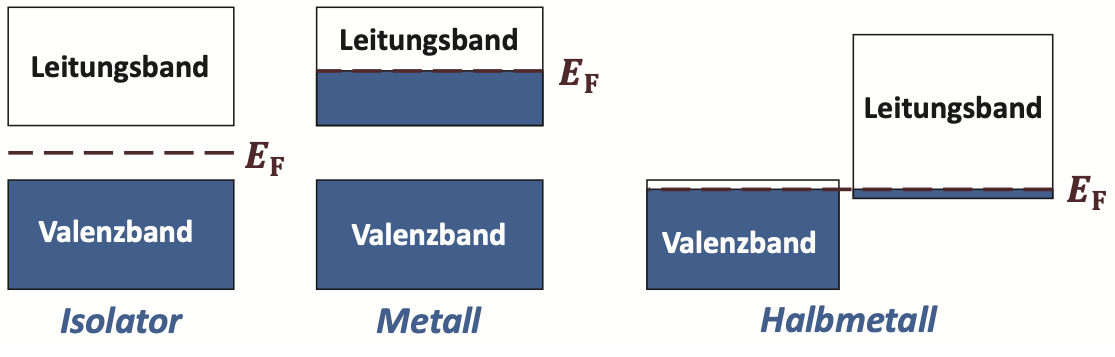
\includegraphics[width=\textwidth]{content/pics/Bandstruktur.png}
    \caption{Bandstruktur eines Isolators, Metalls und Halbmetalls. Hierbei bezeichnet $E_{\symup{F}}$ die Fermienergie \cite{GrossMarx2018}.}
    \label{fig:Bandstruktur}
\end{figure}

\subsection{Effektive Masse}
\label{subsec:Effektive Masse}

\subsection{Zirkulare Doppelbrechung}
\label{subsec:Zirkulare Doppelbrechung}

\begin{figure}
    \centering
    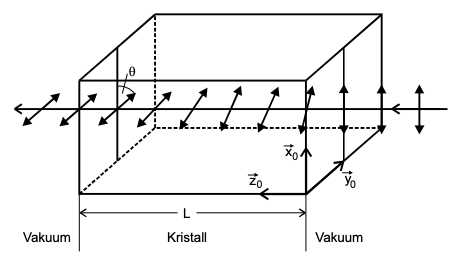
\includegraphics[width=0.8\textwidth]{content/pics/Zirkulare_Doppelbrechung.png}
    \caption{Illustration der zirkularen Doppelbrechung von linear polarisiertem Licht in einem Kristall \cite{V46_Anhang}.}
    \label{fig:Zirkulare Doppelbrechung}
\end{figure}

\subsection{Faraday-Effekt}
\label{subsec:Faraday-Effekt}


\begin{equation}
    \label{eqn:theta_l2}
    \theta_\text{frei} = \frac{e^3 N B}{8\symup{\pi}^2 \varepsilon_0 c^3 (m^*)^2 n} \cdot \lambda^2 
\end{equation}
